%\documentclass{JHEP3}
\documentclass[11pt,a4paper]{article}
\pdfoutput=1
\usepackage{cancel}
\usepackage{enumitem}
\usepackage{etex}
\usepackage{amsthm}
\usepackage{geometry}
\usepackage{dcolumn}
\usepackage{epsf}
\usepackage{mathrsfs}
\usepackage{multirow}
\usepackage{booktabs}
\usepackage{tabularx}
\usepackage{array}
\usepackage{slashed}
\usepackage{float}
\usepackage{leftidx}
\usepackage{setspace}
\usepackage{verbatim}
\usepackage{adjustbox}
\usepackage{tikz}
\usepackage[caption=false]{subfig}
\usepackage{arydshln}
\usepackage{jheppub}
\usepackage{shuffle}
\usepackage{amsmath}
\usepackage{cases}

\numberwithin{equation}{section}
\usetikzlibrary{arrows,decorations.markings,shapes.arrows,patterns,positioning}


\setlength{\oddsidemargin}{0.75in}
\setlength{\evensidemargin}{0.75in} \setlength{\topmargin}{0.75in}
\setlength{\textwidth}{7.0in} \setlength{\textheight}{8.5in}
\renewcommand{\baselinestretch}{1.2}
\jot=2mm

\newcommand{\bea}{\begin{eqnarray}}
\newcommand{\eea}{\end{eqnarray}}
\newcommand{\bean}{\begin{eqnarray*}}
\newcommand{\eean}{\end{eqnarray*}}
\newcommand{\nn}{\nonumber\\}
\newcommand{\Sl}{\sum\limits}
\newcommand{\blue}{\color{blue}}
\newcommand{\red}{\color{red}}
\newcommand{\green}{\color{green}}
\newcommand{\black}{\color{black}}
\def\W #1{\widetilde{#1}}
\def\WH #1{\widehat{#1}}
\def\msout#1{\textrm{\sout{#1}}}
\def\mxout#1{\textrm{\xout{#1}}}
\def\Label#1{\label{#1}%
  \smash{\hbox to0pt{\raise1ex\hbox{\tiny[#1]}\hss}}}
%\def\Label#1{\label{#1}}
\renewcommand{\eqref}[1]{eq.~(\ref{#1})}
%\newcommand{\[1]{eqs.~(\ref{#1})\xspace}
\newcommand{\figref}[1]{Fig.~\ref{#1}}
\newcommand{\tabref}[1]{table~\ref{#1}}
\newcommand{\secref}[1]{section~\ref{#1}}
\newcommand{\appref}[1]{appendix~\ref{#1}}
\newcommand{\tabincell}[2]{\begin{tabular}{@{}#1@{}}#2\end{tabular}}
\def\rightaction#1{\stackrel{\rightarrow}{\partial \over \partial #1}}
\def\leftaction#1{\stackrel{\lefttarrow}{\partial \over \partial #1}}
\def\func#1{\mathop{\rm #1}\nolimits}
\def\abs#1{\left| #1\right|}
\def\braket#1{\left\langle #1 \right\rangle}
\def\bra#1{\left\langle #1\right|}
\def\ket#1{\left| #1\right\rangle}
\def\gb #1{ \left\langle #1 \right]}
\def\tgb #1{ \left[ #1 \right\rangle}
%�����Զ�����%%%%%%%%%%%%%%%%%%%%%%%%%
%\newcommand{\tabincell}[2]{\begin{tabular}{@{}#1@{}}#2\end{tabular}}
%%%%%%%%%%%%%%%%%%%%%%%%%%%%%%%%%%%%%%

\def\Shuffle{{\text{\scriptsize{$\bigsqcup$}}}\mathchoice{\mkern-3mu}{\mkern-3mu}{\mkern-0mu}{\mkern-0mu}{\text{\scriptsize{$\bigsqcup$}}}}


\def\d{\partial}
\def\rmd{{\rm d}}
\def\la{\lambda}
\def\eps{\epsilon}
\def\lblb{({\bar\la}{\bar\la})}
\def\ald{{\dot\alpha}}
\def\bed{{\dot\beta}}
\def\gad{{\dot\gamma}}
\def\sid{{\dot\rho}}
\def\vev{\braket}
\def\tgb #1{ \left[ #1 \right\rangle}
\def\bket#1{\left| #1\right]}
\def\bvev#1{\left[ #1 \right]}
\def\Spaa{\vev}
\def\Spbb{\bvev}
\def\Spab{\gb}
\def\Spba{\tgb}
\def\Sl{\sum\limits}
\def\rchi{\raisebox{\depth}{$\chi$}}
\newcommand{\bbibitem}[1]{\bibitem{#1}\marginpar{#1}}
\newcommand{\ctobedelete}[1]{}
\allowdisplaybreaks

%%%%%%%%%%%%%%%%%%%%%%%%%%%%%%%%%


\title{Topics on scattering amplitudes}

\author[a,b,c]{Yi-Jian Du\footnote{Corresponding author}}


\affiliation[a]{Department of Physics, Wuhan University, No. 299 Bayi Road, Wuhan 430072, China}
\affiliation[b]{College of Science, Tibet University, No.10 Zangda East Road, Lasa, 850000, China}
\affiliation[c]{Suzhou Institute of Wuhan University, No.377 Linquan Street, Suzhou, 215123, China}

\emailAdd{yijian.du@whu.edu.cn}

\date{\today}
\abstract{This note covers various topics of scattering amplitudes, including the new conformal symmetry, off-shell extension of CHY, amplitudes in four dimensions, string theory  and so on.}
\keywords{Amplitude Relation, Gauge invariance}



\begin{document}
\maketitle \flushbottom

\section{Introduction}
I write various new process on scattering amplitudes and problems deserve further study in this note.

\section{Preparations}


\subsection{Decompositions of tree-level GR and color-ordered YM amplitudes}
 {\emph{Gravitons as two copies of gluons}}~~A tree-level scattering amplitude $M^{\text{GR}}(1,2,\dots,n)$ for $n$ gravitons is a rational function of Lorentz contractions of external polarization tensors $\epsilon_i^{\mu\nu}$ ($i=1,\dots,n$) and momenta $k_i^{\mu}$ ($i=1,\dots, n$), where $\epsilon_i^{\mu\nu}$ is a \emph{traceless symmetric tensor} which satisfies
 \bea
 k_{i\,\mu}\epsilon_i^{\mu\nu}=k_{i\,\nu}\epsilon_i^{\mu\nu}=0.
 \eea
In Yang-Mills (YM) theory, an external polarization (of a gluon) $\epsilon_i^{\mu}$ carries only one Lorentz index and satisfies the condition
\bea
k_{i\,\mu}\cdot\epsilon_i^{\mu}=0.
\eea
Thus it seems that a graviton polarization tensor may be written as two copies of gluon polarizations:
 \bea
 \epsilon_i^{\mu\nu}\to \frac{1}{2}(\epsilon_i^{\mu}\widetilde{\epsilon}_i^{\nu}+\epsilon_i^{\mu}\widetilde{\epsilon}_i^{\nu})-\epsilon_i^{\mu}\epsilon_{i\,{\mu}}.\Label{Eq:Polaization1}
 \eea
A polarization $\epsilon_i^{\mu}$ depends on the choice of gauge and the corresponding momentum $k_i^{\mu}$. Once we choose the same gauge for $\epsilon_i^{\mu}$ and $\widetilde{\epsilon}_i^{\nu}$, $\epsilon_i^{\mu}\widetilde{\epsilon}_i^{\nu}$ is naturally a symmetric tensor. Furthermore, in four dimensions, one can always construct YM polarizations such that $\epsilon_i^{\mu}\epsilon_{i\,{\mu}}=0$. In this sense, we will use
 \bea
 \epsilon_i^{\mu\nu}\to\epsilon_i^{\mu}\widetilde{\epsilon}_i^{\nu}\Label{Eq:Polaization2}
 \eea
instead of \eqref{Eq:Polaization1}. In the following, all gravitons and gluons are treated as massless particles, thus we always have $k_i^2=0$ if we are considering the \emph{on-shell amplitudes}. Another condition for momenta is momentum conservation $\Sl_{i=1}^nk_i^{\mu}=0$.

{\emph{Decompositions of GR and YM amplitudes}}~~Tree-level scattering amplitudes for $n$ gravitons can be written as
%
\bea
M^{\text{GR}}(1,2,\dots,n)=\Sl_{\pmb{\sigma}\in S_{n-2}}N_{1|\pmb{\sigma}|n}A^{\text{YM}}(1,\pmb{\sigma},n), \Label{Eq:ExpansionGR}
\eea
%
where $N_{1,\pmb{\sigma},n}$ are called BCJ numerators in DDM basis. In the above equation, $A^{\text{YM}}(1,\pmb{\sigma},n)$ denote color-ordered YM amplitudes, while $\pmb{\sigma}$ denote the $(n-2)!$ permutations (i.e. an element in $S_{n-2}$) of the external particles $2,3,\dots,n-1$. In general, the numerator $N_{1|\pmb{\sigma}|n}$ is a rational function of $k_i\cdot k_j$, $\epsilon_i\cdot k_j$ and $\epsilon_i\cdot\epsilon_j$, while the other copies of polarizations $\widetilde{\epsilon_i}$ are included in the color ordered YM amplitudes $A^{\text{YM}}(1,\pmb{\sigma},n)$.
A BCJ numerator $N_{1|\pmb{\sigma}|n}$ does not have unique form because it is gauge dependent.

A color-ordered YM amplitude $A^{\text{YM}}(1,\pmb{\sigma},n)$ can be decomposed similarly:
%
\bea
A^{\text{YM}}(1,\pmb{\sigma},n)=\Sl_{\pmb{\rho}\in S_{n-2}}\widetilde{N}_{1|\pmb{\rho}|n}A^{\text{BS}}(1,\pmb{\sigma},n|1,\pmb{\rho},n). \Label{Eq:ExpansionYM}
\eea
%
Here $\widetilde{N}_{1|\pmb{\rho}|n}$ (the other copy of BCJ numerator) is a  function of Lorentz contractions $\widetilde{\epsilon_i}\cdot \widetilde{\epsilon_j}$, $\widetilde{\epsilon_i}\cdot {k_j}$ and $k_i\cdot k_j$. $\widetilde{N}_{1|\pmb{\rho}|n}$ can be constructed by a same rule with ${N}_{1|\pmb{\rho}|n}$. The amplitude $A^{\text{BS}}(1,\pmb{\rho},n)$ is called bi-scalar amplitude which depends on both permutations $\pmb{\sigma}$ and $\pmb{\rho}$ and does not contain any polarization.


Inserting the \eqref{Eq:ExpansionYM} into the gravity amplitude \eqref{Eq:ExpansionGR}, we get
\bea
M^{\text{GR}}(1,2,\dots,n)=\Sl_{\pmb{\sigma}\in S_{n-2}}\Sl_{\pmb{\rho}\in S_{n-2}}N_{1|\pmb{\sigma}|n}A^{\text{BS}}(1,\pmb{\sigma},n|1,\pmb{\rho},n)\widetilde{N}_{1|\pmb{\rho}|n}, \Label{Eq:ExpansionGR1}
\eea
which expresses a gravity amplitude $M^{\text{GR}}(1,2,\dots,n)$ by bi-scalar ones associated with two copies of BCJ numerators. Apparently, information of all polarizations are included in the BCJ numerators.

\subsection{The rule for bi-scalar amplitudes}

\begin{figure}
\centering
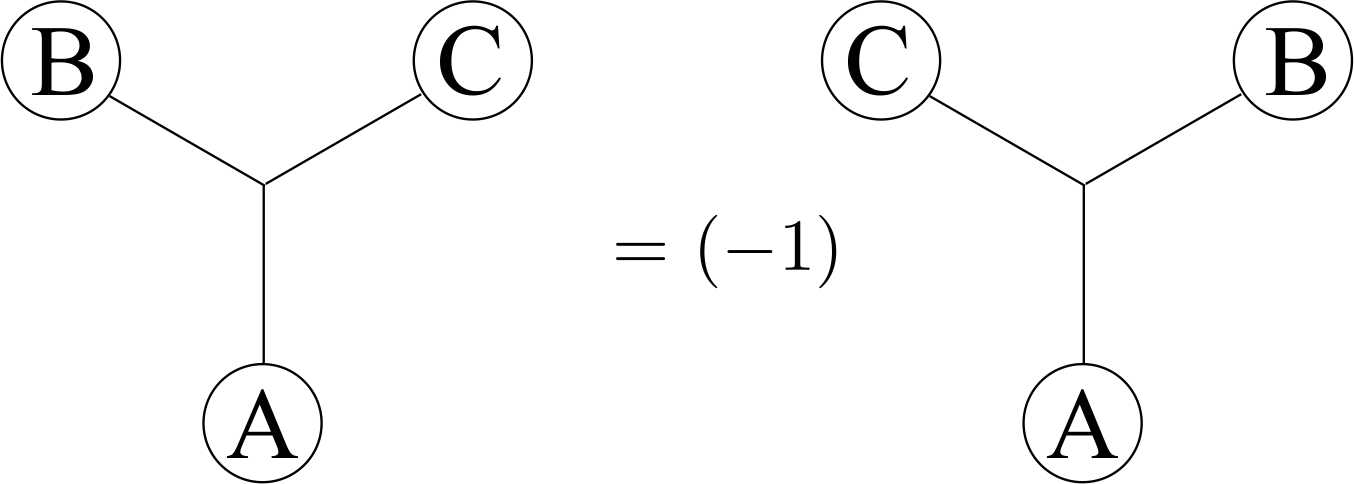
\includegraphics[width=0.5\textwidth]{Sign.jpg}
\caption{Two graphs which are related by exchanging two branches attached to a same cubic vertex must have opposite signs.}\label{Fig:Sign}
\end{figure}

\begin{figure}
\centering
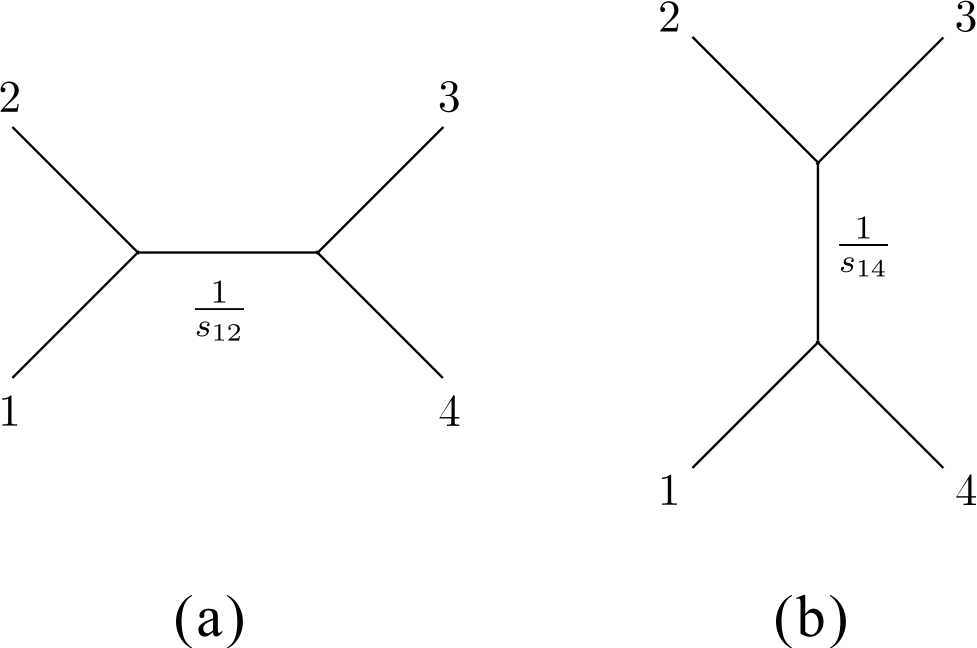
\includegraphics[width=0.5\textwidth]{BS4pt.jpg}
\caption{Both (a) and (b) are Feynman diagrams for $A^{\text{BS}}(1,2,3,4|1,2,3,4)$. Only (b) is allowed by $A^{\text{BS}}(1,2,3,4|1,3,2,4)$.}\label{Fig:BS4pt}
\end{figure}

Now we present the construction rule for bi-scalar amplitudes $A^{\text{BS}}(1,\pmb{\sigma},n|1,\pmb{\rho},n)$. A bi-scalar amplitude is given by summing over all possible \emph{trivalent Feynman diagrams} (i.e. diagrams constructed by only \emph{cubic vertices}) that are allowed by both permutations $1,\pmb{\sigma},n$ and $1,\pmb{\rho},n$. Each diagram contributes the product of propagators therein, with a proper sign. The sign is determined as follows: if two diagrams contribute the same propagators, they must be related by exchanging branches attached to cubic vertices. Such an exchanging introduces a minus sign (see \figref{Fig:BS4pt}). Consequently, if the number of such exchangings is even, the sign should be $(+1)$, otherwise, (-1).

Let us take the four-point BS amplitudes as  examples. For the amplitude $A^{\text{BS}}(1,2,3,4|1,2,3,4)$, $\pmb{\sigma}=\pmb{\rho}=\{2,3\}$. The  Feynman diagrams allowed by both permutations are shown by \figref{Fig:BS4pt} (a) and (b). Therefore, the amplitude is
\bea
A^{\text{BS}}(1,2,3,4|1,2,3,4)={1\over s_{12}}+{1\over s_{14}}.
\eea
Here, $s_{ij}\equiv (k_i+k_j)^2=2k_i\cdot k_j$.

Another four-point amplitude $A^{\text{BS}}(1,2,3,4|1,3,2,4)$ is only given by \figref{Fig:BS4pt} (b). This is because \emph{(i)} both diagrams (a) and (b) in \figref{Fig:BS4pt} are allowed by the permutation $1,2,3,4$ \emph{(ii)} the diagrams \figref{Fig:BS4pt} (a), (b) when exchanging $2\leftrightarrow3$ are those allowed by the permutation $1,3,2,4$. The common diagram of \emph{(i)} and \emph{(ii)} is only \figref{Fig:BS4pt} (b) (although for (ii), we should exchange $2$ and $3$ in \figref{Fig:BS4pt} (b), it contributes the same propagator ${1\over s_{14}}$). The exchanging number is $1$ for \figref{Fig:BS4pt} (b). Thus
\bea
A^{\text{BS}}(1,2,3,4|1,3,2,4)=-{1\over s_{14}}.
\eea
{\color{blue}\bf Exercise-1~~~~What are the Feynman diagrams for the following five-point bi-scalar amplitudes:
\newline
$A^{\text{BS}}(1,2,3,4,5|1,2,3,4,5)$, $A^{\text{BS}}(1,4,3,2,5|1,3,2,4,5)$ and $A^{\text{BS}}(1,2,3,4,5|1,4,3,2,5)$? Calculate these amplitudes.}

\subsection{Refined graphic rule for GR and color-ordered YM amplitudes}
Instead of presenting a construction rule for the BCJ numerators with a permutation $\pmb{\sigma}$ explicitly (although we are able to do this), we provide another expression of GR amplitude here:
%
\bea
M^{\text{GR}}(1,2,\dots,n)=\Sl_{\mathcal{F}}C^{[\mathcal{F}]}\biggl[\,\Sl_{\pmb{\sigma}^{\mathcal{F}}}A^{\text{YM}}(1,\pmb{\sigma}^{\mathcal{F}},n)\biggr], \Label{Eq:ExpansionGR}
\eea
%
where all possible refined graphs $\mathcal{F}$ have been summed over. For each graph, we have \emph{(i)} a coefficient $C^{[\mathcal{F}]}$ which is a polynomial of factors $k_i\cdot k_j$, $\epsilon_i\cdot \epsilon_j$ and $\epsilon_i\cdot\epsilon_j$, \emph{(ii)} a sum of amplitudes with permutations $\pmb{\sigma}^{\mathcal{F}}$ that are allowed by this graph. When $M^{\text{GR}}(1,2,\dots,n)$ on the LHS is replaced by the color-ordered YM amplitude $A^{\text{YM}}(1,\pmb{\sigma},n)$ and $A^{\text{YM}}(1,\pmb{\sigma}^{\mathcal{F}},n)$ on the RHS is replaced by the bi-scalar amplitude $A^{\text{BS}}(1,\pmb{\sigma}^{\mathcal{F}},n|1,\pmb{\rho},n)$, the expression \eqref{Eq:ExpansionGR} becomes an expansion of YM amplitudes. We will explain the coefficients $C^{[\mathcal{F}]}$ and permutations $\pmb{\sigma}^{\mathcal{F}}$ in detail.
\begin{figure}
\centering
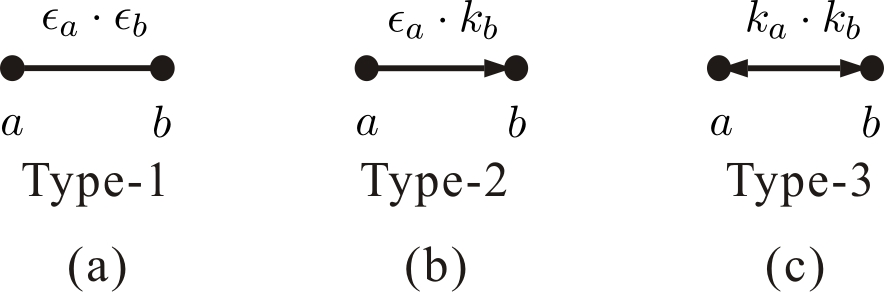
\includegraphics[width=0.45\textwidth]{Lines.jpg}
\caption{Line styles}\label{Fig:Lines}
\end{figure}
\begin{figure}
\centering
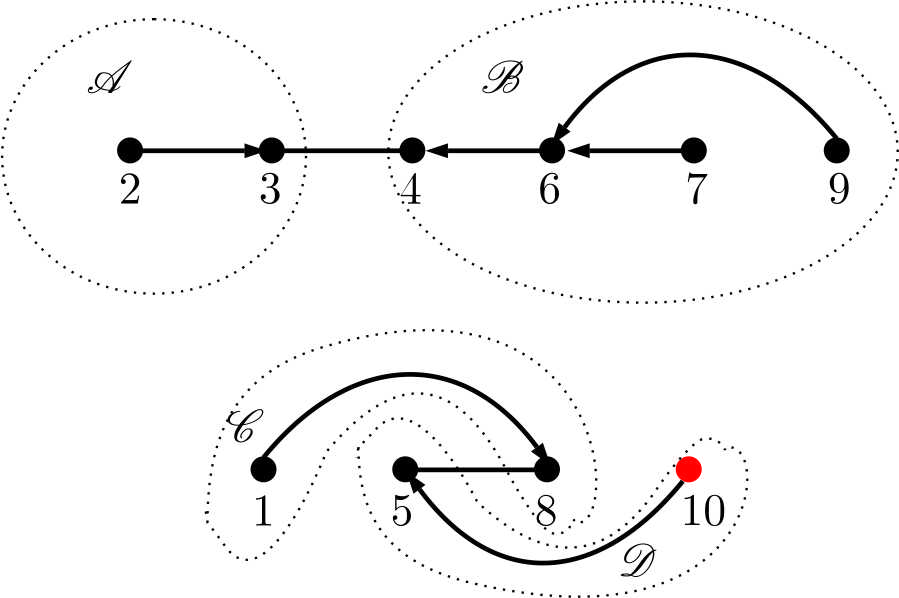
\includegraphics[width=0.45\textwidth]{Components.jpg}
\caption{}\label{Fig:Components}
\end{figure}

~~~~~~~~~~~~~~~~~~~~~~~~~~~~~~~~~~~~~~~~~~~~~~~{\bf\emph{Refined graphic rule}}

{\bf\emph{Reference order}}~~~Consider each graviton as a node, define a reference order
\bea
\mathsf{R}=\{1,\rho(1),...,\rho(n-1),n\},\Label{Eq:ReferenceOrder}
 \eea
 where the two gravitons $1$ and $2$ are considered as the first and the last elements in $\mathsf{R}$ (of cause, you can chose other two elements instead). The permutation $\pmb{\rho}\equiv\{\rho(2),\rho(3),\dots,\rho(n-1)\}$ is an arbitrary permutation of $2$, $3$, ..., $n-1$. The position of each element in $\mathsf{R}$ is called its \emph{weight}. Apparently, $n$ is the highest-weight element and $1$ is the lowest-weight one in $\mathsf{R}=\{1,\rho(1),...,\rho(n-1),n\}$.

{\bf\emph{ Nodes and line styles}}~~~Every external particle is considered as a node. To construct a graph, we need to connect lines between nodes. There are three types of lines \figref{Fig:Lines} (a), (b) and (c) which correspond to factors $\epsilon_a\cdot\epsilon_b$, $\epsilon_a\cdot k_b$ and $k_a\cdot k_b$.


{\bf\emph{The construction of graphs}}~~Graphs are constructed as follows:
\begin{itemize}
\item [\bf\emph{(i)}]{\bf Grouping nodes}~~We divide the gravitons $1,\dots,n$ into several sets such that \emph{(a)} the highest- and the lowest-weight elements in the reference order \eqref{Eq:ReferenceOrder} are always in a same group, \emph{(b)} every group must contains at least two elements.
    {\color{blue}\bf Exercise-2:~~Supposing that the reference order for $4$-point amplitude is $\mathsf{R}=\{1,2,3,4\}$, what are the possible groupings?}
\item [\bf\emph{(ii)}] {\bf Constructing components for each group of elements}~~Given a grouping, {\bf for the set containing the highest-weight and the lowest-weight elements $1$, $n$} (for example the set $\{1,5,8,10\}$ in \figref{Fig:Components}), find out a path (which may passes through other nodes in this group) from $n$ to $1$ (for example the path in \figref{Fig:Components} is $10\to 5\to 8\to 1$) and connect arbitrary two adjacent nodes on this path via a type-1 line (for example the nodes $5$ and $8$ are connected by a type-1 line), which is called the \emph{kernel}. Any other pair of adjacent nodes on this path are connected by a type-2 line (\figref{Fig:Lines} (b)) whose arrow points to the kernel (for example, the $1$,$8$ nodes and the $10$, $5$ nodes are connected by type-2 lines (with arrows pointing to the kernel) respectively). We also connect other nodes in this set arbitrarily via type-2 lines pointing towards those nodes ({\bf except the node $n$}) on the path from $n$ and $1$. Then all nodes in this set form a \emph{fully connected tree graph, which is called a component}. \emph{For a set which does not contain $1$ and $n$} (for example the set $\{2,3,4,6,7,9\}$ in \figref{Fig:Components}), pick out arbitrary two elements (in \figref{Fig:Components} the elements $3$ and $4$) and connect them by a type-1 line (the kernel). Other nodes in this set point towards the kernel via type-2 lines in an arbitrary way. Then nodes in this set also form a fully connected tree graph (a \emph{component}). A graph with a given grouping and a given configuration of components for each set in this grouping is called a \emph{skeleton} (for example, \figref{Fig:Components} is a skeleton for $10$-point amplitude). Apparently, each skeleton consists of at least one component. {\color{blue}\bf Exercise-3:~~Find out all possible skeletons for four-point amplitudes.}

\item [\bf\emph{(iii)}] {\bf Weights of components, the top and the bottom sides of components}~~Each component is separated into two parts by its kernel. We define the \emph{top side} by the part which containing the highest-weight node in this component. The opposite side is called the \emph{bottom side}. For example, if the reference order is defined by the regular order $\mathsf{R}=\{1,2,3,\dots,9,10\}$, the top side of components containing $2,3,4,6,7,9$ in \figref{Fig:Components} is the part $\mathscr{B}$, while the bottom side is the part $\mathscr{A}$. The top side of the component containing $1,5,8,10$ is $\mathscr{D}$, while the bottom side is $\mathscr{C}$. We define the \emph{weight of each component} by the weight of its highest-weight node.



\item [\bf\emph{(vi)}] {\bf From skeletons to fully connected graphs}~~If a skeleton has only one component, it is already a connected graph. If a skeleton consists of more than one mutually disjoint components, we should connect these components, via type-3 lines, in a proper way to form a fully connected tree graph. 
    \begin{itemize}
    \item {\bf\emph{Step-1}}, we arrange those components, which does not contain $1$ and $n$, into an ordered set $\mathsf{R}^{\mathscr{C}}=\{\mathscr{C}_1,\mathscr{C}_1,\dots,\mathscr{C}_N\}$ (the reference order for components) according to their weights. We define the component containing the node $1$ as the root part $\mathcal{R}$. 
        
    \item {\bf\emph{Step-2}} Pick out the highest weight component $\mathscr{C}_N$ and other components $\mathscr{C}_{i_1},\dots,\mathscr{C}_{i_j}$ arbitrarily and construct a chain of components towards the root part $\mathsf{R}^{\mathscr{C}}$ as follows:
    %
    \bea
    \mathbb{CH}=\Bigl[(\mathscr{C}_N)_{t}-(\mathscr{C}_N)_{b}\leftrightarrow(\mathscr{C}_{i_j})_{t(\text{\,or\,}b)}-(\mathscr{C}_{i_j})_{b(\text{\,or\,}t)}\leftrightarrow\dots\leftrightarrow(\mathscr{C}_{i_1})_{t(\text{\,or\,}b)}-(\mathscr{C}_{i_1})_{b(\text{\,or\,}t)}\leftrightarrow\mathcal{R}\setminus\{n\}\Bigr].\Label{Eq:Chain}\nn
    \eea
    %
    Here, a subscript $t$ or $b$ denotes the top or bottom side of the corresponding component. The notation `$-$' between two sides of a component denotes the kernel. A `$\leftrightarrow$' denotes the type-3 line between two nodes in the corresponding regions. For example the `$\leftrightarrow$' between $(\mathscr{C}_N)_{b}$ and $(\mathscr{C}_{i_j})_{t(\text{\,or\,}b)}$ means that we connect arbitrary nodes $x$, $y$ ($x\in (\mathscr{C}_N)_{b}, y\in (\mathscr{C}_{i_j})_{t(\text{\,or\,}b)}$) by a type-3 line. $\mathcal{R}\setminus\{n\}$ is used to recall that $n$ cannot be considered as a root. {\bf Note that all the kernels of the components $\mathscr{C}_N,\mathscr{C}_{i_j},\dots,\mathscr{C}_{i_1}$ in \eqref{Eq:Chain} on this chain are passed through by the path that starts from the highest-weight element in $\mathscr{C}_N$ and ends at the node $1$!} After this construction, we redefine the reference order $\mathsf{R}^{\mathscr{C}}$ and the root part $\mathcal{R}$:
    \bea
    \mathsf{R}^{\mathscr{C}}\to \mathsf{R}^{\mathscr{C}}\setminus\{\mathscr{C}_1,\mathscr{C}_1,\dots,\mathscr{C}_N\}, \mathcal{R}\to \mathcal{R}\cup \{\mathscr{C}_1,\mathscr{C}_1,\dots,\mathscr{C}_N\}.
    \eea
\item {\bf \emph{Step-3}} Repeating Step-2 until the ordered set $\mathsf{R}^{\mathscr{C}}$ becomes empty. Then a fully connected graph is produced.
\end{itemize}
\end{itemize}
{\bf All possible graphs (i.e. all possible groupings, all possible skeletons for a given grouping, all possible graphs constructed from a given skeleton) produced along the above line together are all graphs $\mathcal{F}$ in \eqref{Eq:ExpansionGR}!} {\color{blue}\bf Exercise-4:~~Construct all possible graphs for $4$-point amplitudes! (Hint: classify the graphs according to the number of components. Although the above construction rule seems very complicated, it is not hard to treat the $4$-point case.)} 


{\bf\emph{The factor $C^{[\mathcal{F}]}$ and permutations $\pmb{\sigma}^{\mathcal{F}}$}}  The factor $C^{[\mathcal{F}]}$ is given by the product of all lines (defined by \figref{Fig:Lines}) inside a graph with a proper sign $(-1)^{\mathcal{N}(\mathcal{F})}$ where $\mathcal{N}(\mathcal{F})$ is the total number of arrows pointing away from the node $1$. The permutations $1,\pmb{\sigma}^{\mathcal{F}},n$ are determined by: (i) $1$ and $n$ are always considered as the first and the last elements, (ii) if $x$ and $y$ are two adjacent elements and $x$ is nearer to the node $1$ than $y$, the relative orders of them must satisfy $(\pmb{\sigma}^{\mathcal{F}})^{-1}(x)<(\pmb{\sigma}^{\mathcal{F}})^{-1}(y)$ \footnote{Here we use $\sigma^{-1}(x)$ to denote the position of $x$ in the permutation $\pmb{\sigma}$}. (iii) If two substructures are attached to a same node, we should \emph{shuffle} the permutations corresponding to these two substructures together. As an example, if we connect the nodes $3$ and $8$ in \figref{Fig:Components} via a type-3 line, the factor $C^{[\mathcal{F}]}$ is given by 
\bea
\Bigl[(-\epsilon_1\cdot k_8)(\epsilon_5\cdot\epsilon_8)(\epsilon_{10}\cdot k_5)\Bigr](k_3\cdot k_8)\Bigl[(\epsilon_2\cdot k_3)(\epsilon_3\cdot\epsilon_4)(\epsilon_6\cdot k_4)(\epsilon_9\cdot k_6)(\epsilon_7\cdot k_6)\Bigr]
\eea
and the permutations $\pmb{\sigma}^{\mathcal{F}}$ are given by 
\bea
\pmb{\sigma}^{\mathcal{F}}\in\Bigl\{\{8,5\}\shuffle\{3,\{2\}\shuffle\{4,6,\{9\}\shuffle\{7\}\}\}\Bigr\}.
\eea
{\color{blue}\bf Exercise-5:~~Write down the coefficients $C^{[\mathcal{F}]}$ and all amplitudes $A(1,\pmb{\sigma}^{\mathcal{F}},n)$ for all the graphs $\mathcal{F}$ constructed in Exercise-4}.


\section{New conformal symmetry}




\section{On off-shell extension}


\section{One-loop amplitudes}

\section{String amplitudes}
 \bibliographystyle{JHEP}
\bibliography{NoteONGaugeIdentity}

\end{document}
